\documentclass[conference]{IEEEtran}
%\IEEEoverridecommandlockouts
% The preceding line is only needed to identify funding in the first footnote. If that is unneeded, please comment it out.
\usepackage{cite}
\usepackage{amsmath,amssymb,amsfonts}
\usepackage{algorithmic}
\usepackage{graphicx}
\usepackage{textcomp}
\usepackage{xcolor}
\usepackage{hyperref}
\renewcommand\labelenumi{[\theenumi].}

\begin{document}

\title{Investigating image embeddings}

\author{
\IEEEauthorblockN{Arezou Ranjbarpour Maralani}
\IEEEauthorblockA{\textit{arezo.ranjbarpour@gmail.com}}
\and
\IEEEauthorblockN{Lorenzo Tibaldi}
\IEEEauthorblockA{\textit{chio999@hotmail.it}}
\and
\IEEEauthorblockN{Momina Sajid}
\IEEEauthorblockA{\textit{momnabutt058@gmail.com}}
}

\maketitle

\begin{abstract}
In this project we took a closer look to different famous models trained on the imagenet dataset,
intermediate features and their representation in 3D space and reasoned about one particular metric: the Silhouette score.
\end{abstract}

\begin{IEEEkeywords}
image embedding, imagenet, 3D visualization, intermediate features, silhouette score, transfer learning.
\end{IEEEkeywords}

\section{Introduction}
Transfer learning is a tecnique that involves taking advantage of a pretrained model,
creating intermediate features of the datapoints to create an \emph{Image Embedding} and then
utilizing a much simpler model to fine tune the classification according to your needs.

\section{Implementation}

\subsection{The Dataset}
We decided to use a dataset downloaded from kaggle\footnote{Aviable here: \url{https://www.kaggle.com/andrewmvd/animal-faces}},
It contains thousands of pictures of animal faces: cats, dogs and "Wildlife".

We added 6 possible labels, previously grouped in the class "Wildlife":
fox, cheetah, lion, tiger, wolf and leopard, and kept the 2 other original classes: cat and dog.

We then reduced the number of images that we were going to use and also resized them from 512x512 to
200x200 for computational reasons.

One thing to note is that those animals were all present in the imagenet possible classes, and as such it
should yield, in theory, very good results and at most generate a bigger error in the classes cat and dog because
there is a much bigger intraclass variance in those species (even if most "Wildlife" datapoints contained some 
"whiter" variants like the arctic fox or the white tiger).

\subsection{The Models}
We experimented with most of the models that Keras offerred that didn't exceed 100 MB in size (again for computational reasons).

In \ref{ModelTable} we compare the sizes of the different models, how many intermediate features they have as output 
and how long it takes to produce those new embedded datapoints from our input images. 

\begin{table*}[htbp]
\caption{Models used for Image Embedding}
\begin{center}
\begin{tabular}{|c|c|c|c|c|}
\hline
\textbf{Name} &\textbf{Model Size} &\textbf{Number of Parameters} & \textbf{Number of Features} &\textbf{Average Execution Time}\\
\hline
\hline
Xception [\ref{1}] & 88MB & 22,910,480 & 100,352 &  16.4s\\
\hline
ResNet50V2 [\ref{2}] & 98MB & 25,613,800 & 100,352 & 24.8s\\
\hline
InceptionV3 [\ref{3}] & 92MB & 23,851,784 & 32,768 &  10.2s\\
\hline
MobileNetV2 [\ref{4}] & 14MB & 3,538,984 & 62,720  & 9.5s\\
\hline
DenseNet201 [\ref{5}] & 80MB & 20,242,984 & 69,120 & 56.1s\\
\hline
\end{tabular}
\label{ModelTable}
\end{center}
\end{table*}

All the models were initialized with the imagenet weigths.

\subsection{The top layers}
The very top layers are the parts that get fine tuned for the classification problem at hand.

This model contains only:
\begin{itemize}
\item{A Flatten layer, to accept the intermediate features.}
\item{A BatchNormalization layer, to speed up convergence.}
\item{A first Dense layer with ReLU as activation function and 512 neurons.}
\item{A dropout layer with a drop out factor of 50\%, to avoid overfitting.}
\item{A last Dense layer with softmax activation function and as many neurons as possible labels, to solve our multi class classification problem.}
\end{itemize}
The model is then compiled with sparse categorical crossentropy as loss and told to keep track of loss and accuracy of both the training and validation set.

During training we gave a conservative number of epochs for the model to improve, we wanted to show that transfer learning starts good and becomes
better pretty fast, as expected all the training accuracies start above 60\% (the majority above 88\%), and then improve to excellent in one or two epochs, with the exception of the DenseNet201 that would've probably improved to a much better result had we given it more epochs to work with.

\section{First Results}
\subsection{Classification}
The first results (shown in \ref{ResTable}) were the accuracies of the fine tuned model obtained on the test set after using the different intermediate features that the pre-trained models returned as inputs.

It can also be seen as an estimation of how good those intemediate features are since the easier the datapoints are to separate the better the final accuracy would be.

By comparing \ref{ModelTable} and \ref{ResTable} we are able to say something more:
\begin{itemize}
\item{InceptionV3 gave the best result for our dataset.}
\item{InceptionV3 is also the model that returns the least amount of intermediate features, probably highlighting how, for our dataset, we didn't need too many features.}
\item{It would, however, be wrong to deduce that having more features decreases accuracy because the DenseNet201 model was the worst model but exactly in the middle as far as number of features go.}
\item{There is no direct correlation between the number of parameters or features and the execution time for these pre-trained model.}
\item{We have been surprised by the performance of MobileNetV2, a model that performed very well and yet needs very little space on disk, few parameters in comparison to the other models and has the best execution time for the Image Embedding.}
\end{itemize}

\begin{table}[htbp]
\caption{Performance of Transfer Learning}
\begin{center}
\begin{tabular}{|c|c|c|}
\hline
\textbf{Name} &\textbf{Average Loss} &\textbf{Average Accuracy}\\
\hline
\hline
Xception [\ref{1}] & 0.5231 & 99.3\%\\
\hline
ResNet50V2 [\ref{2}] & 0.6525 & 98.4\%\\
\hline
InceptionV3 [\ref{3}] & \textbf{0.0449} & \textbf{99.8\%}\\
\hline
MobileNetV2 [\ref{4}] & 0.3981 & 99.1\%\\
\hline
DenseNet201 [\ref{5}] & 1.0198 & 85.7\%\\
\hline
\end{tabular}
\label{ResTable}
\end{center}
\end{table}

\subsection{Exploring Intermediate Features}
Then it is possible to take a look at the intermediate features by applying a dimensionality reduction algorithm.

What we would expect is being able to identify clusters of points that are easily separable in 3D space whenever the accuracy of the model is very high.

In this part we utilized 2 very well known dimensionality reduction methods: PCA and T-SNE, Figures \ref{Xception_3d}, \ref{ResNet_3d}, \ref{Inception_3d} \ref{MobileNet_3d} and \ref{DenseNet_3d} show the results obtained.\footnote{The visualizations are rotated in one of the best possible viewpoints, however it might still be difficult to tell exactly what is happening by only using a still image.}

With the exception of the DenseNet201 model, all the features are more or less clearly separable, as the excellent results in \ref{ResTable} would suggest, the T-SNE result for the MobileNetV2 features is a bit anomalous but the elongated clusters are still pretty separable.

It is important to note however that this is a 3D reduction of a much bigger feature space, even the messy DenseNet201 result was able to be separated correctly more than 80\% of the time when all the features were considered.

\section{Evaluating Intermediate Features}
\subsection{Silhouette Score definition}
At this point it's possible to wonder about the performance of the clustering, for example by using the silhouette score [\ref{6}]:
\begin{equation}
S(i) = \frac{b(i) - a(i)}{max\{a(i),b(i)\}}
\label{sil}
\end{equation}
where \emph{a(i)} (\ref{a}) is the average distance of point \emph{i} from all the points in its correct cluster
and \emph{b(i)} (\ref{b}) is the average distance of point \emph{i} from all the points in the closest cluster it doesn't belong.

\begin{equation}
a(i) =\frac{1}{|C_{i}| - 1} \sum_{\substack{
   j \in C_{i} \\
   j \neq i
  }} d(i,j)
\label{a}
\end{equation}
\begin{equation}
b(i) = \min_{k \neq i} \frac{1}{|C_{k}|} \sum_{j \in C_{k}} d(i,j)
\label{b}
\end{equation}
Defining C as the set of clusters: $C = \{{c_{0},c_{1},c_{2} \dots}\}$, $C_{i}$ as the cluster that \emph{i} belongs to 
and $d(i,j)$ as the multidimensional distance between the coordinates of the two points considered.

Silhouette scores range from -1 to 1, points with a Silhouette score closer to 1 are correctly and "tightly" clustered and the ones closer to -1 are either very distant from their cluster or roughly in the center of a wrong one.

Considering that each point has a score it is natural to just calculate a simple average of the whole dataset and show the results for each model.

\subsection{Silhouette Score Results}
Results for both PCA and T-SNE are shown for every model in \ref{ScoreTable}.

\begin{table*}[hbpt]
\caption{Performance of Dimensionality Reduction}
\begin{center}
\begin{tabular}{|c|c|c|c|c|}
\hline
\textbf{Model} &\multicolumn{2}{|c|}{\textbf{PCA}} &\multicolumn{2}{|c|}{\textbf{T-SNE}}\\
\cline{2-5}
\textbf{Name} &\textbf{Average Execution Time} &\textbf{Average Silhouette Score} &\textbf{Average Execution Time} &\textbf{Average Silhouette Score}\\
\hline
\hline
Xception [\ref{1}] & 13.1s & \textbf{0.6790} & 32m 10s & 0.4964\\
\hline
ResNet50V2 [\ref{2}] & 12.6s & 0.5187 & 32m 10s & \textbf{0.5079}\\
\hline
InceptionV3 [\ref{3}] & \textbf{3.86s} & 0.6747 & \textbf{11m 18s} & 0.4824\\
\hline
MobileNetV2 [\ref{4}] & 7.40s & 0.5156 & 21m 22s & 0.4508\\
\hline
DenseNet201 [\ref{5}] & 8.12s & -0.0384 & 23m 23s & 0.0288\\
\hline
\end{tabular}
\label{ScoreTable}
\end{center}
\end{table*}

Some questions that might come to mind are: Why didn't the InceptionV3 model give the best results? And why did the best result for PCA and T-SNE belong to different models even if applied to the same data?

The answer for the first question is that the results in \ref{ResTable} start from the intermediate features but then depend on the training of the top model,  in the same way the results in \ref{ScoreTable} start from the same intermediate features but then depend on the dimensionality reduction algorithms, so we can say that maybe the Xception and ResNet50V2 features had some "low importance values" that might have "confused" (in a very minor way) the classifier but then when picking only the 3 most descriptive ones it turns out that they are more descriptive than the 3 best ones from InceptionV3.

It should be possible in theory to train the model on the features \textbf{after} dimensionality reduction, and then it would be possible to see a linear correlation between accuracies and silhouette scores.

The answer to the second question lies in how differently PCA and T-SNE work, as it can be deduced even with no knowledge of the algorithms just by looking at the execution times, it can be correctly assumed that PCA is much simpler than T-SNE but it would be incorrect to say that the T-SNE results are better because T-SNE can apply some distortion on top of the loss of information that PCA also does since we are just selecting 3 principal components [\ref{7}]. 

By comparing \ref{ModelTable} and \ref{ScoreTable} we can again deduce that the execution times of the dimensionality reduction algorithms scale with the number of intermediate features, processing around 8200 features per second in PCA and 50 features per second in T-SNE.

It is also possible to compare \ref{ResTable} and \ref{ScoreTable} and deduce that there isn't a linear correlation between accuracy and Silhouette Score but it is clear by the DenseNet201 results that a low Silhouette Score (in this case close to 0) leads to a lower accuracy.

\section{Working on the pre-trained models}
\subsection{Fine Tuning}
Even if the results are very good as is, it is possible to fine tune the final layers of the pre-trained models, doing so would in theory generate Intermediate Features that are more specific to our dataset.

For this purpose we decided to retrain all the layers from the last convolutional one until the end.

It is very important to set the learning rate much smaller than the default, so that our top layer wouldn't "throw off" the last layers of the pre-trained models.
\subsection{Results}
The table \ref{FineTable} contains all the results obtained and the difference of the previous executions that can be found in the other tables, in Figure \ref{Xception_fine}, \ref{ResNet_fine}, \ref{Inception_fine}, \ref{MobileNet_fine}, \ref{DenseNet_fine} the new position of the features are shown.

In theory fine tuning should always improve the models, however our models had a very good accuracy to begin with, additionally it's possible that the huge size of the last convolutional layers (regarding the number of parameters) required a very big dataset to be tuned properly, it is probable that we would've obtained a better result just by having more data.

An exceptional offender is the model that actually had the best accuracy before: InceptionV3, that worsened quite a bit.

Still it's worth noting that the DenseNet201 model actually improved, an educated guess might be that the model wasn't completely fit yet and giving some additional epochs to the last layer turned out to be desirable.

Finally it is also interesting how the accuracies mostly worsened but the silhouette scores didn't, at least not as much, this might be explained by highlighting how fine tuning the last convolutional layer might have increased the importance of some features that were already important, prompting the dimensionality reduction algorithms to ignore less important features and revelaing a more tightly clustered visualization.

\begin{table*}[htbp]
\caption{Performance of Fine Tuning}
\begin{center}
\begin{tabular}{|c|c|c|c|c|c|c|c|c|}
\hline
& \multicolumn{4}{|c|}{\textbf{\ref{ResTable}}} & \multicolumn{4}{|c|}{\textbf{\ref{ScoreTable}}}\\
\cline{2-9}
\textbf{Model} & \textbf{Average} && \textbf{Average} && \multicolumn{2}{|c|}{\textbf{PCA}} &\multicolumn{2}{|c|}{\textbf{T-SNE}}\\
\cline{6-9}
\textbf{Name} & \textbf{Loss} & \textbf{Difference} & \textbf{Accuracy} & \textbf{Difference} & \textbf{Silhouette Score} & \textbf{Difference} & \textbf{Silhouette Score} & \textbf{Difference}\\     
\hline
\hline
Xception [\ref{1}] & \textbf{0.5933} & +0,0702 & \textbf{97.5\%} & -1.8\% & \textbf{0.6580} & -0.0210 & 0.4279 & -0.0685\\
\hline
ResNet50V2 [\ref{2}] & 0.8142 & +0.1617 & 94.2\% & -4.2\% & 0.5039 & -0.0148 & \textbf{0.4891} & -0.0188\\
\hline
InceptionV3 [\ref{3}] & 1.8663 & +1.8214 & 81.2\% & -18.6\% & 0.3397 & -0.3350 & 0.3822 & -0.1002\\
\hline
MobileNetV2 [\ref{4}] & 0.7157 & +0.3176 & 95.1\% & -4.0\% & 0.5180 & +0.0024 & 0.4849 & +0.0341\\
\hline
DenseNet201 [\ref{5}] & 0.8095 & \textbf{-0.2103} & 92.9\% & \textbf{+7.2\%} & 0.5801 & \textbf{+0.6185} & 0.4404 & \textbf{+0.4116}\\
\hline
\end{tabular}
\label{FineTable}
\end{center}
\end{table*}

\section{Doing more with Silhouette Score}
One could then ask themselves if it's possible to use the silhouette score to do something more?

We are going to present the theory behind what can be done, but we encountered some technical issues during implementation of the code for it.

In theory it would be possible to create a new model that takes in input the features (either before or after dimensionality reduction) and that performs some sort of regression were it's trying to predict the best place to "move" the datapoint so that the silhouette score is maximized.

The model would then be trained using a variation of the silhouette score as loss, so the best results come from minimizing instead of maximizing, this variation can be as simple as (\ref{l}), so that when the point is perfectly clustered the loss is 0 and when completely misclustered the loss is 1.

\begin{equation}
L(i) = \frac{S(i) - 1}{-0.5}
\label{l}
\end{equation}

It is not exactly obvious when the "moving" of the points would happen, meaning at which point would the predictions be used in the future silhouette score calculation, the very nature of this metric is a bit unusual because it's somewhat both local and global, local because it describes any point, but global because by itself it needs the position of all the other points.

For completeness we want to point out that the model \emph{could} be created with a target in mind even when doing clustering, the points could be told to converge towards the centroid of the cluster that they really belong to (this is exploiting a huge advantage that we have because our problem is not \textbf{only} clustering, and as such we can introduce some supervised learning tricks).

Doing so only on the training set would teach to the model a transformation that might not even be what we want, for example if the majority of the points in the training set would need to be moved towards the positives on the x axis and the majority of the points belonging to the same cluster in the test set would need to be moved towards the negatives on the x axis the model might increase the distance of those points from the centroid during the final prediction.

If, to avoid that anomalous transformation, the centroids are created from an union of the training and test set then it's easy to see that not only that would defeat the purpose of the clustering but also of the classification, since we are basically creating a lookup table with the coordinates of the centroids on one side and the correct classes on the other.

Assuming a correct implementation of the previous steps, the result would just be a transformation of the Image Embeddings of the pre-trained models into a different Image embedding that might consider a lower amount of "coordinates" in the feature space.

At this point the results are for all intents and purposes intermidiate features and can be fed to the classification model like we did in the rest of the paper.

\section{Final considerations}
In this project we explored the Image Embedding of many pre-trained models, took advantage of them for some transfer learning and fine tuning, then compared some results and drawn some connections between the moving parts, we also gave some consideration to the Silhouette Score that is a metric we had never seen before, probably because it's domain is unsupervised learning.

The whole project was developed in Python on Google Collaboratory mainly utilizing the Keras library, all the material can be found on GitHub here: \url{https://github.com/WeLikeIke/ComputationalVision_Project}

\begin{figure}
\centerline{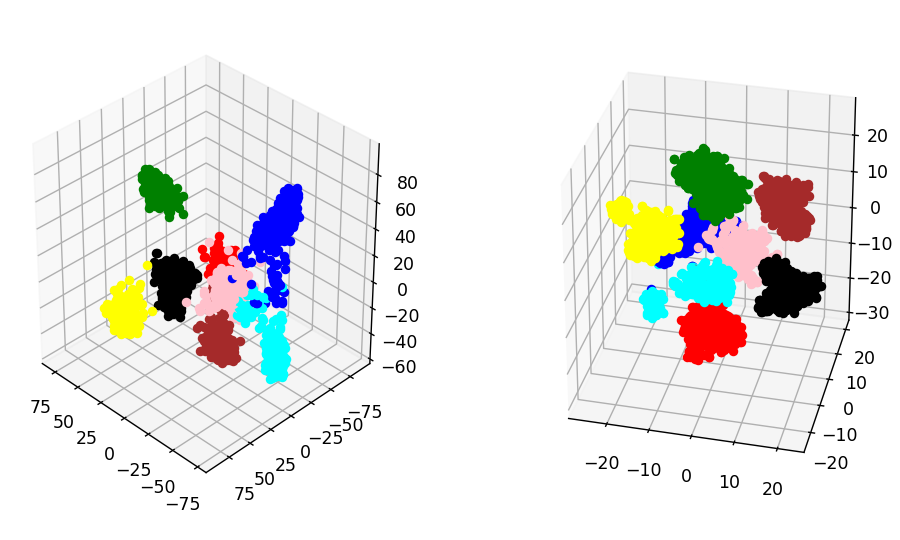
\includegraphics[width=0.45\textwidth]{Xception_3d}}
\caption{results of PCA on the left and T-SNE on the right for the output of the Xception model.}
\label{Xception_3d}
\end{figure}
\begin{figure}[htbp]
\centerline{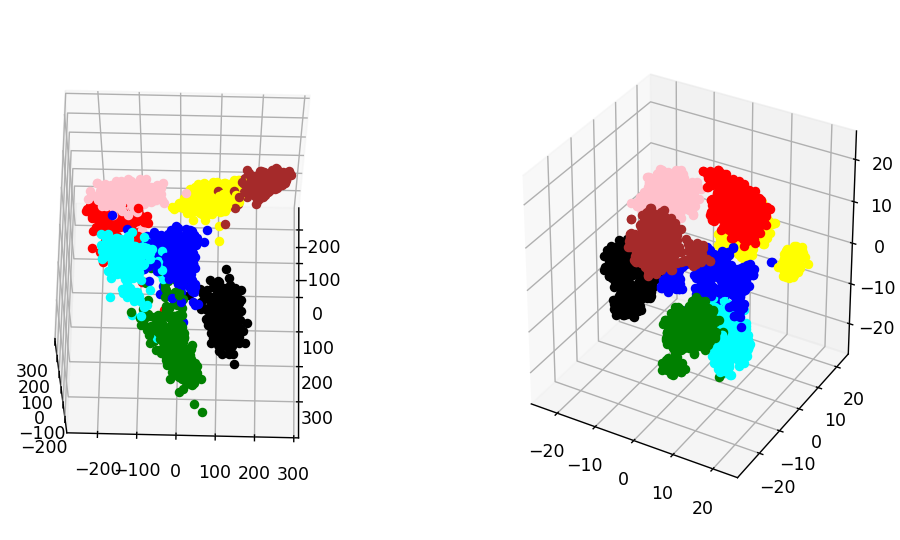
\includegraphics[width=0.45\textwidth]{ResNet_3d}}
\caption{results of PCA on the left and T-SNE on the right for the output of the ResNet50V2 model.}
\label{ResNet_3d}
\end{figure}
\begin{figure}[htbp]
\centerline{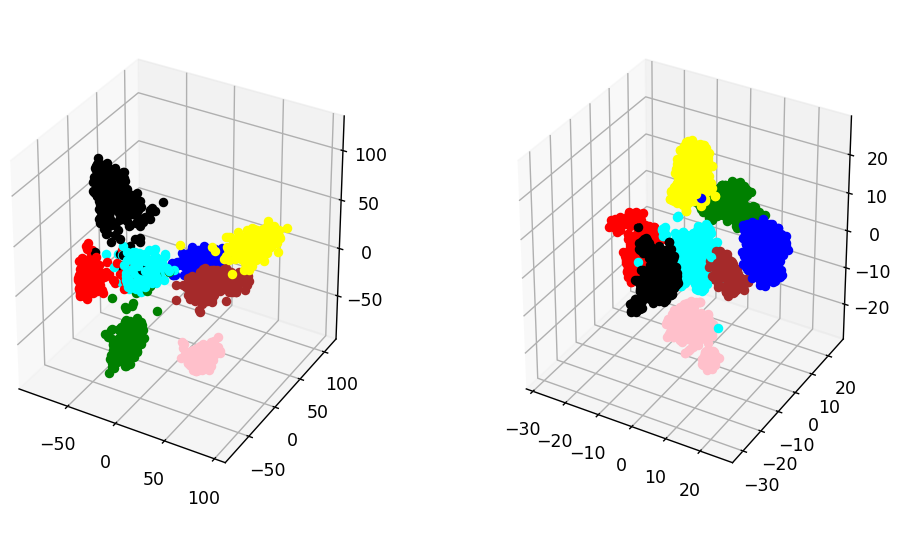
\includegraphics[width=0.45\textwidth]{Inception_3d}}
\caption{results of PCA on the left and T-SNE on the right for the output of the InceptionV3 model.}
\label{Inception_3d}
\end{figure}
\begin{figure}[htbp]
\centerline{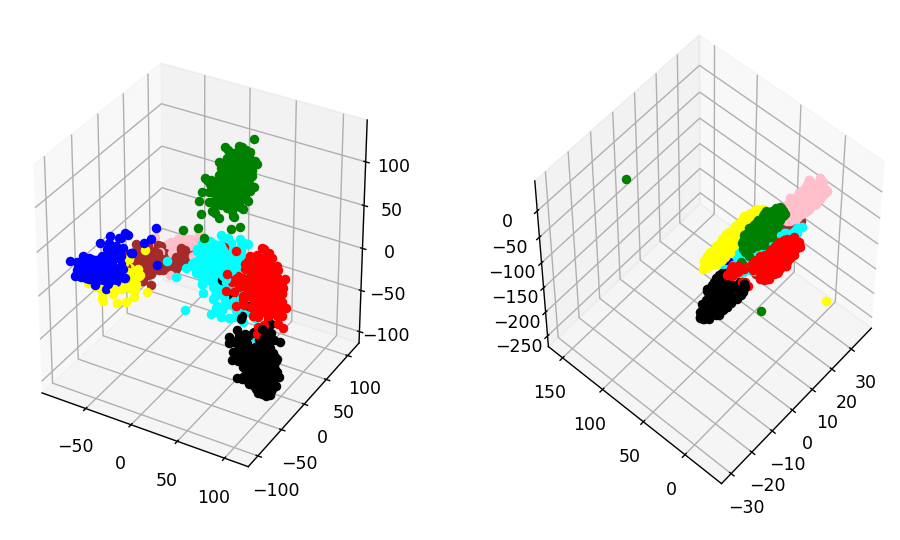
\includegraphics[width=0.45\textwidth]{MobileNet_3d}}
\caption{results of PCA on the left and T-SNE on the right for the output of the MobileNetV2 model.}
\label{MobileNet_3d}
\end{figure}
\begin{figure}[htbp]
\centerline{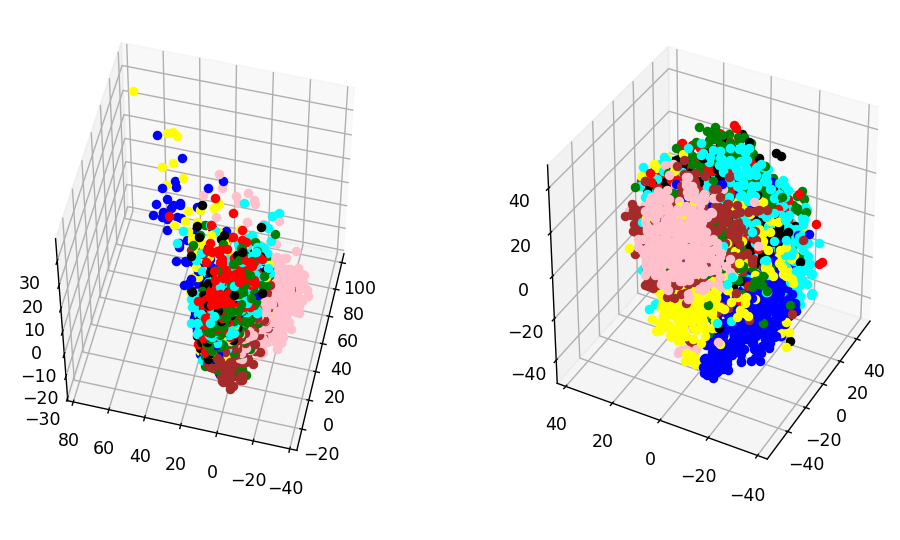
\includegraphics[width=0.45\textwidth]{DenseNet_3d}}
\caption{results of PCA on the left and T-SNE on the right for the output of the DenseNet201 model.}
\label{DenseNet_3d}
\end{figure}

\begin{figure}
\centerline{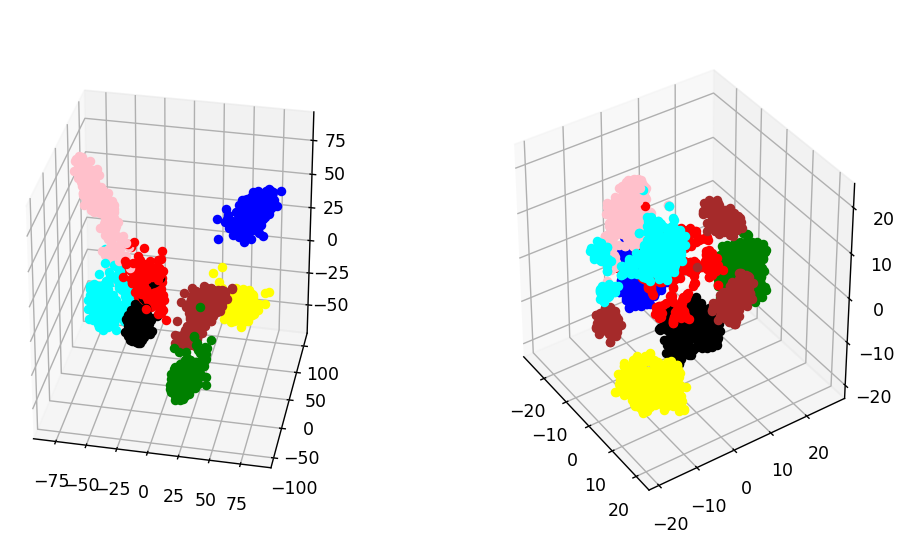
\includegraphics[width=0.45\textwidth]{Xception_fine}}
\caption{results of PCA on the left and T-SNE on the right for the output of the tuned Xception model.}
\label{Xception_fine}
\end{figure}
\begin{figure}[htbp]
\centerline{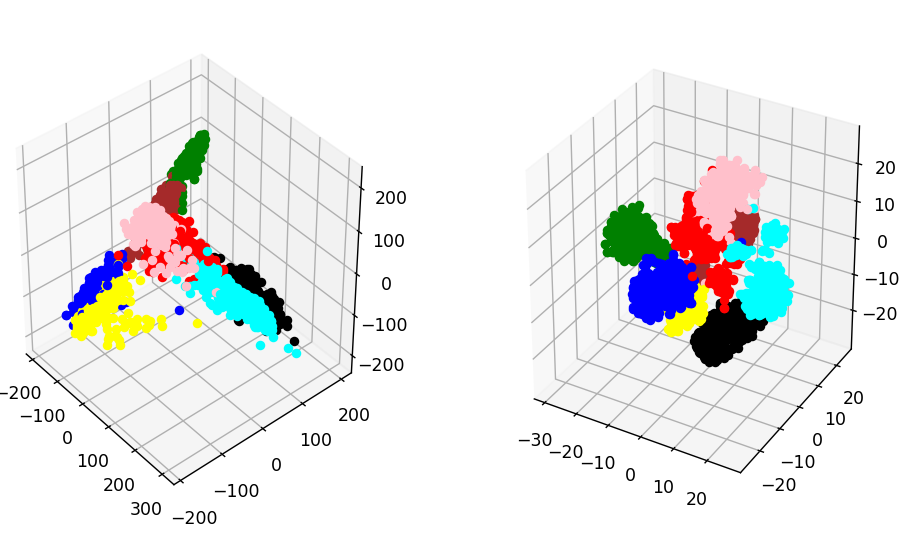
\includegraphics[width=0.45\textwidth]{ResNet_fine}}
\caption{results of PCA on the left and T-SNE on the right for the output of the tuned ResNet50V2 model.}
\label{ResNet_fine}
\end{figure}
\begin{figure}[htbp]
\centerline{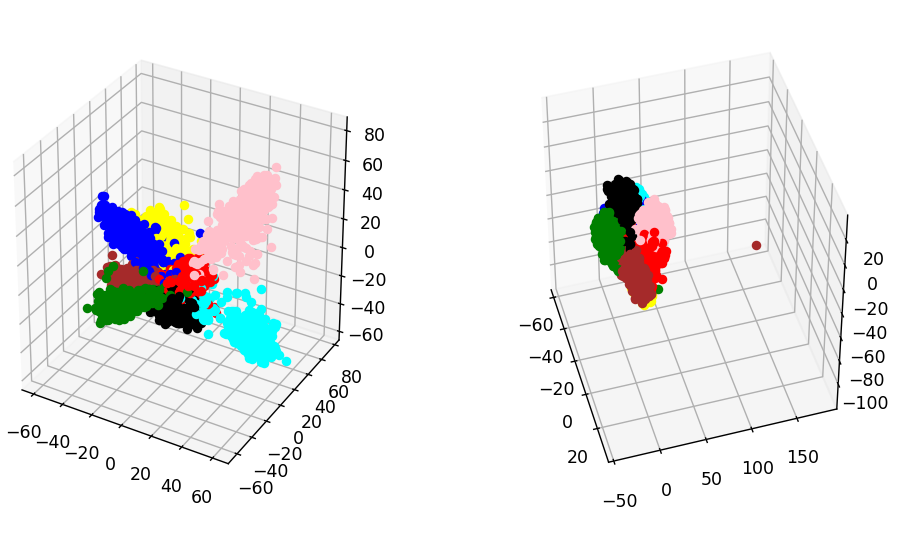
\includegraphics[width=0.45\textwidth]{Inception_fine}}
\caption{results of PCA on the left and T-SNE on the right for the output of the tuned InceptionV3 model.}
\label{Inception_fine}
\end{figure}
\begin{figure}[htbp]
\centerline{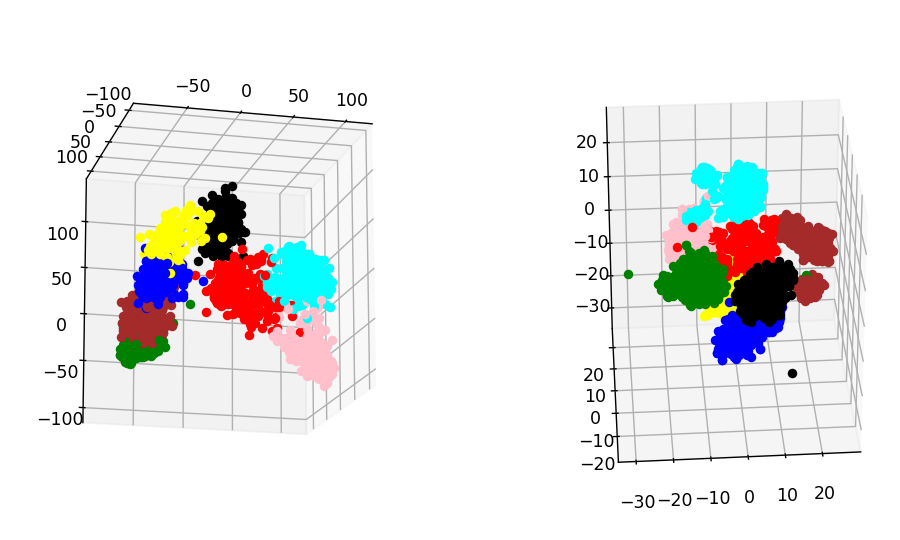
\includegraphics[width=0.45\textwidth]{MobileNet_fine}}
\caption{results of PCA on the left and T-SNE on the right for the output of the tuned MobileNetV2 model.}
\label{MobileNet_fine}
\end{figure}
\begin{figure}[htbp]
\centerline{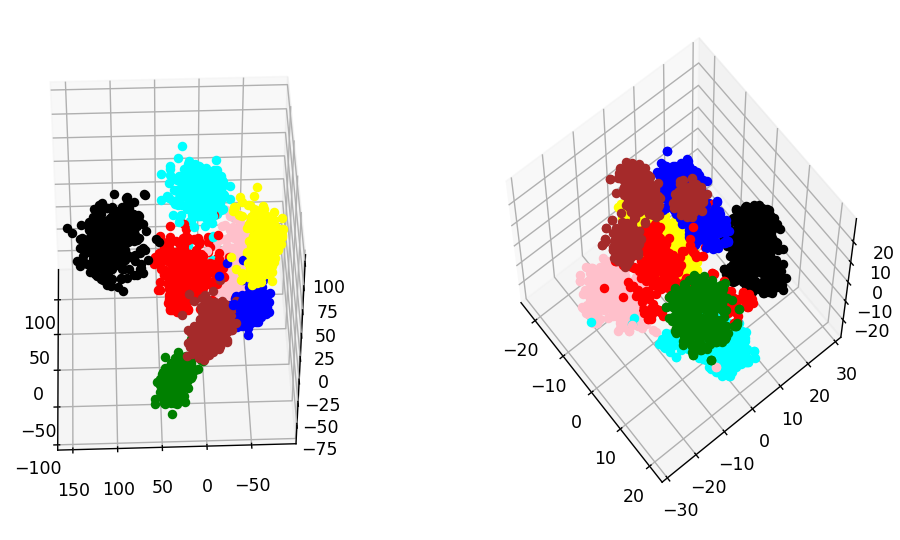
\includegraphics[width=0.45\textwidth]{DenseNet_fine}}
\caption{results of PCA on the left and T-SNE on the right for the output of the tuned DenseNet201 model.}
\label{DenseNet_fine}
\end{figure}


\clearpage
\section*{References}
\begin{enumerate}
\item{\url{https://arxiv.org/pdf/1610.02357.pdf} \label{1}}
\item{\url{https://arxiv.org/pdf/1603.05027.pdf} \label{2}}
\item{\url{https://arxiv.org/pdf/1512.00567.pdf} \label{3}}
\item{\url{https://arxiv.org/pdf/1801.04381.pdf} \label{4}}
\item{\url{https://arxiv.org/pdf/1608.06993.pdf} \label{5}}
\item{\url{https://medium.com/@ODSC/assessment-metrics-for-clustering-algorithms-4a902e00d92d} \label{6}}
\item{\url{https://distill.pub/2016/misread-tsne/}\label{7}}
\end{enumerate}
\end{document}
